\chapter{Fundamentação Teórica}
\label{cap:fund}

\section{Definições Principais}

Para melhor esclarecer os assuntos abordados, é importante que seja primeiramente definido alguns dos termos centrais para a fundamentação do trabalho.

\subsection{Qualidade de Serviço}

Qualidade de serviço é uma métrica sistêmica que sumariza o quão bem o sistema provisiona suas funcionalidades em um determinado momento. É possível definir e modelar essa métrica de diversas maneiras, mas para os propósitos deste trabalho, será utilizada uma definição simples que resume a funcionalidade geral numa escala de 0 a 1.

A qualidade de serviço $Q$ do sistema pode ser aproximada pela média ponderada de seus serviços $S_0 ... S_n$ com os pesos de seus fatores de contribuição para a qualidade total $q_0 ... q_n$ \cite{SchedAndOptOfDistributedFT}.

\begin{equation}
    Q = \frac{ \sum^{i = 0}_{n} S_i q_i }{ \sum^{i = 0}_{n} q_i}
\end{equation}
\addEquacao{Qualidade de Serviço}{1}


\subsection{Falhas}

De acordo com a definição de anormalidades de software da IEEE: um erro (\textit{error}) é a diferença entre um valor esperado e o valor obtido. Um defeito (\textit{fault}) é um estado irregular do sistema que pode (ou não) provocar erros que resultem em falhas. Já uma falha (\textit{failure}) é uma incapacidade observável do sistema de cumprir sua função designada, constituindo uma degradação total ou parcial de sua qualidade de serviço \cite{IEEEAnormalities}.

Neste trabalho, o termo "falha" será utilizado de forma mais geral, representando um estado ou evento no sistema que cause uma degradação na sua qualidade de serviço.

\subsubsection{Padrões de Ocorrência}

Falhas podem ser classificadas em 3 grupos principais quanto ao seu padrão de ocorrência \cite{FaultTolerantSystems}.

\begin{itemize}
    \item Falhas Transientes: Ocorrem aleatoriamente e possuem um impacto temporário.

    \item Falhas Intermitentes: Assim como as transientes possuem duração e impacto temporários, porém ocorrem periodicamente.

    \item Falhas Permanentes: Causam uma degradação permanente no sistema da qual não pode ser recuperada, potencialmente necessitando de intervenção externa.
\end{itemize}

\subsection{Dependabilidade}

Será utilizado o termo dependabilidade como uma propriedade que sumariza os atributos:  confiabilidade, disponibilidade, capacidade de manutenção e segurança (conhecidos em inglês como critérios RAMS. Os critérios serão definidos na seção seguinte.

A tolerância à falhas impacta positivamente os critérios confiabilidade e disponibilidade, e pode em alguns casos melhorar a capacidade de manutenção, sendo assim, a tolerância à falhas é um aspecto importante para sistemas com boa dependabilidade.

\subsubsection{Confiabilidade}

Confiabilidade (\textit{Reliability}), é a probabilidade de um sistema executar corretamente no período $[t_0, t]$. Para modelar essa métrica é necessário um modelo estatístico que é particular da aplicação. A confiabilidade $R$ é uma função do tempo $t$, a taxa de falhas $\lambda$ e quaisquer sejam os outros parâmetros do modelo \cite{FaultInjectionTechniques}.

\begin{equation}
    R(t) = f(t, \lambda, ...)
\end{equation}
\addEquacao{Confiabilidade}{2}

\subsubsection{Disponibilidade}

Disponibilidade (\textit{Availability}) é a razão entre o tempo em que o sistema não consegue prover seu serviço (\textit{downtime}) e o e seu tempo total de operação \cite{FaultInjectionTechniques}. A disponibilidade $A$ pode ser modelada em termos do tempo disponível $t_{up}$ e do tempo indisponível $t_{down}$:

\begin{equation}
    A = t_u / (t_{up} + t_{down})
\end{equation}
\addEquacao{Disponibilidade}{3}

\subsubsection{Capacidade de manutenção}

Capacidade de manutenção (\textit{Maintainability}) é a probabilidade de um sistema em um estado inválido ser reparado com sucesso antes de um tempo $t$ \cite{FaultInjectionTechniques}.

A modelagem deste atributo necessita de conhecimento particular sobre a aplicação e sobre a disponibilidade de equipamentos ou especialistas humanos para a realização do reparo. Pode ser definida como uma função probabilidade do tempo $t$, taxa de falhas $\lambda$ e os outros parâmetros do modelo.

\begin{equation}
    M(t) = f(t, lambda, ...)
\end{equation}
\addEquacao{Capacidade de Manutenção}{4}

\subsubsection{Segurança}

Segurança (\textit{Safety}) é a probabilidade do sistema não causar danos à integridade humana ou à outros patrimônios, independentemente da presença falhas. Por ser um critério muito particular da natureza da aplicação e seu contexto de operação, uma estimativa analítica necessita de um modelo estatístico que não é facilmente sumarizado com apenas uma equação \cite{FaultInjectionTechniques}.






\section{Tolerância à Falhas}

\subsection{Mecanismos de Detecção}

Mecanismos de detecção são responsáveis por identificar a presença de uma falha no sistema, um bom mecanismo de detecção deve ser capaz de detectar uma classe grande de falhas sem introduzir uma penalidade grande ao tempo de execução do sistema. Dentre as possíveis escolhas de mecanismos, os subsequentes são utilizados neste trabalho.

\subsubsection{CRC (Cyclic Redundancy Check)}

Os CRCs são códigos de detecção de erro comumente utilizados em redes de computador e armazenamento não volátil. Para cada segmento de dado é concatenado um valor de checagem que é calculado com base no resto da divisão com um polinômio gerador pré definido \cite{FaultTolerantSystems}.

CRCs são comumente utilizados devido à serem simples de implementar, ocuparem pouco espaço adicional no segmento e serem resilientes à "burst errors", falhas transientes que alteram uma região de bits próximos.
% TODO: Botar uma figura do payload com um crc

\subsubsection{Heartbeat signals}
% TODO Mencionar sobre como eles botem ser usados pra checar o critério real time

Os heartbeat signals (sinais de batimento cardíaco) são sinais periódicos para garantir a atividade de um nó computacional com o recebimento de uma resposta, são também chamados de "watchdog timers" \cite{DependabilityInEmbeddedSystems}. 

\begin{figure}[H]
    \centering
    \caption{Sequência de um Heartbeat Signal}
    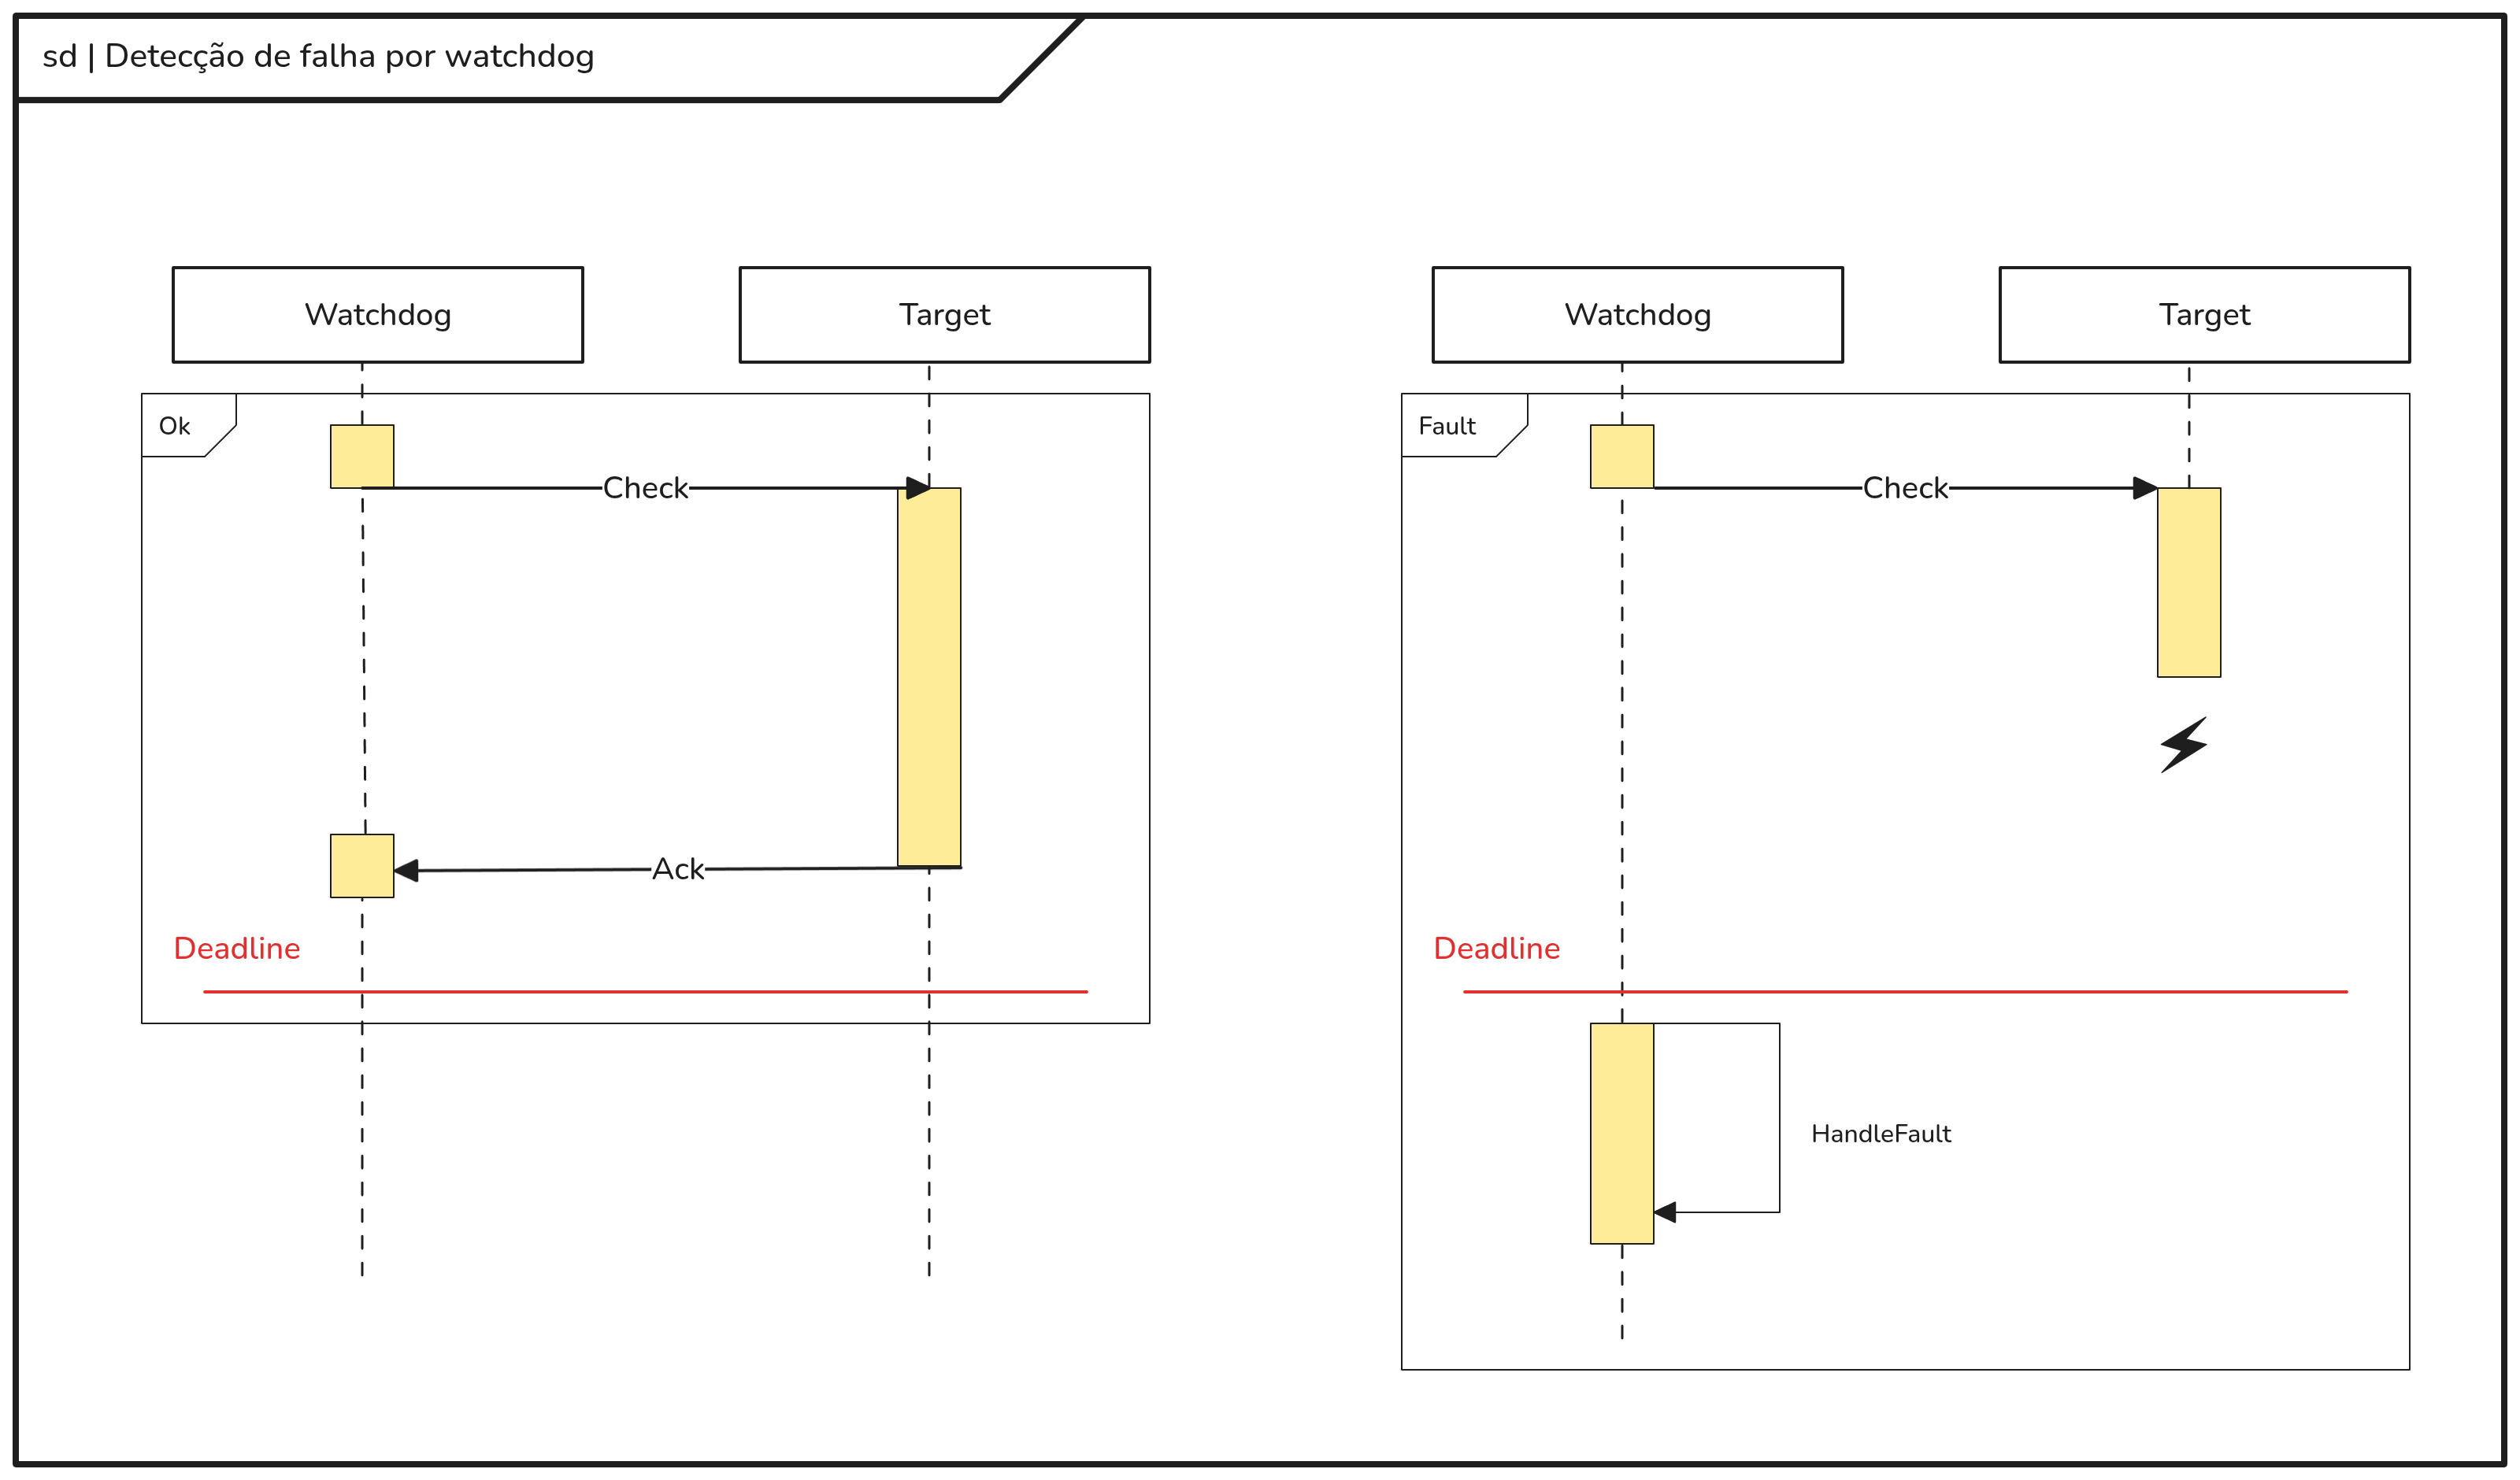
\includegraphics[width=1.0\textwidth]{assets/heartbeat_signal.png}\\
    \caption*{Fonte: Elaborada pelo autor}
    \label{fig:heartbeatSignal}
\end{figure}

Na \autoref{fig:heartbeatSignal}, é utilizado a resposta tardia para deduzir a presença de uma falha na tarefa ou no canal de transmissão. Estes sinais também podem ser utilizados no contexto de tempo real para a validação de um prazo ou sub prazo da tarefa @FaultTolerantSystems. 

\subsubsection{Asserts}

Asserts são mecanismos simples e flexíveis para a detecção de falhas, consistindo na verificação de uma condição que, durante uma execução normal do programa, deve permanecer invariavelmente verdadeira (denominada "invariante"). Caso a invariante seja falsa, detecta-se a presença de uma falha. A \autoref{fig:assert} ilustra o fluxo de um assert.

% TODO(marcos): Fluxograma de um assert

Apesar de sua simplicidade, quando usados em conjunto com simulações determinísticas e ferramentas de \textit{fuzzer} asserts podem tanto detectar erros durante a execução assim como revelar erros de design durante a fase de desenvolvimento \cite{TigerBeetleSafety} \cite {PowerOf10Rules}.

% TODO(marcos): citar Spark e ou C3 pre/post conditions
Durante a execução de um sistema tolerante à falhas, asserts servem como uma forma de saber rapidamente que algo errado aconteceu. Porém não são robustos o suficiente para detectar corrupção silenciosa de dados ou pulos inesperados de maneira consistente. Quando asserts são inseridos na entrada ou saída de um procedimento são denominados como pré-condições e pós-condições respectivamente. Alguns compiladores são capazes de automaticamente inserir estas condições para assegurar contratos da interface de um programa.

\subsection{Mecanismos de Tratamento}

Uma vez que uma falha tenha sido detectada o sistema precisa tratar a falha o mais rápido possível para manter a qualidade de serviço, alguns mecanismos de detecção também fornecem a possibilidade de correção dos dados, como é o caso dos códigos Reed-Solomon, nestes casos, fica à critério da aplicação se a correção deve ser tentada ou outro tratamento deve ser usado.

\subsubsection{Re-execução}

Re-executar uma tarefa é uma outra forma simples de recuperar-se de uma falha, a probabilidade de $k$ falhas intermitentes ocorrem em sequência é menor do que a probabilidade de apenas ocorrer $k - 1$ vezes no intervalo de execução. Ao re-executar, espera-se que a falha não ocorra novamente na N-ésima tentativa. \cite{DependabilityInEmbeddedSystems}

Portanto, é sacrificado um tempo maior de execução caso a falha ocorra, em troca de um tempo menor de execução médio sem necessitar de componentes extras. Em contraste com a técnica de redundância tripla, é possível entender que a redundância tripla ou "tradicional", depende de uma resiliência "espacial" (É improvável que uma falha ocorra em vários lugares ao mesmo tempo), enquanto a re-execução depende de uma resiliência "temporal" (É improvável que múltiplas falhas ocorram repetidamente em $N$ execuções) % TODO(marcos): citar aqui eh importante

\begin{figure}[H]
    \centering
    \caption{Exemplo de reexecuções}
    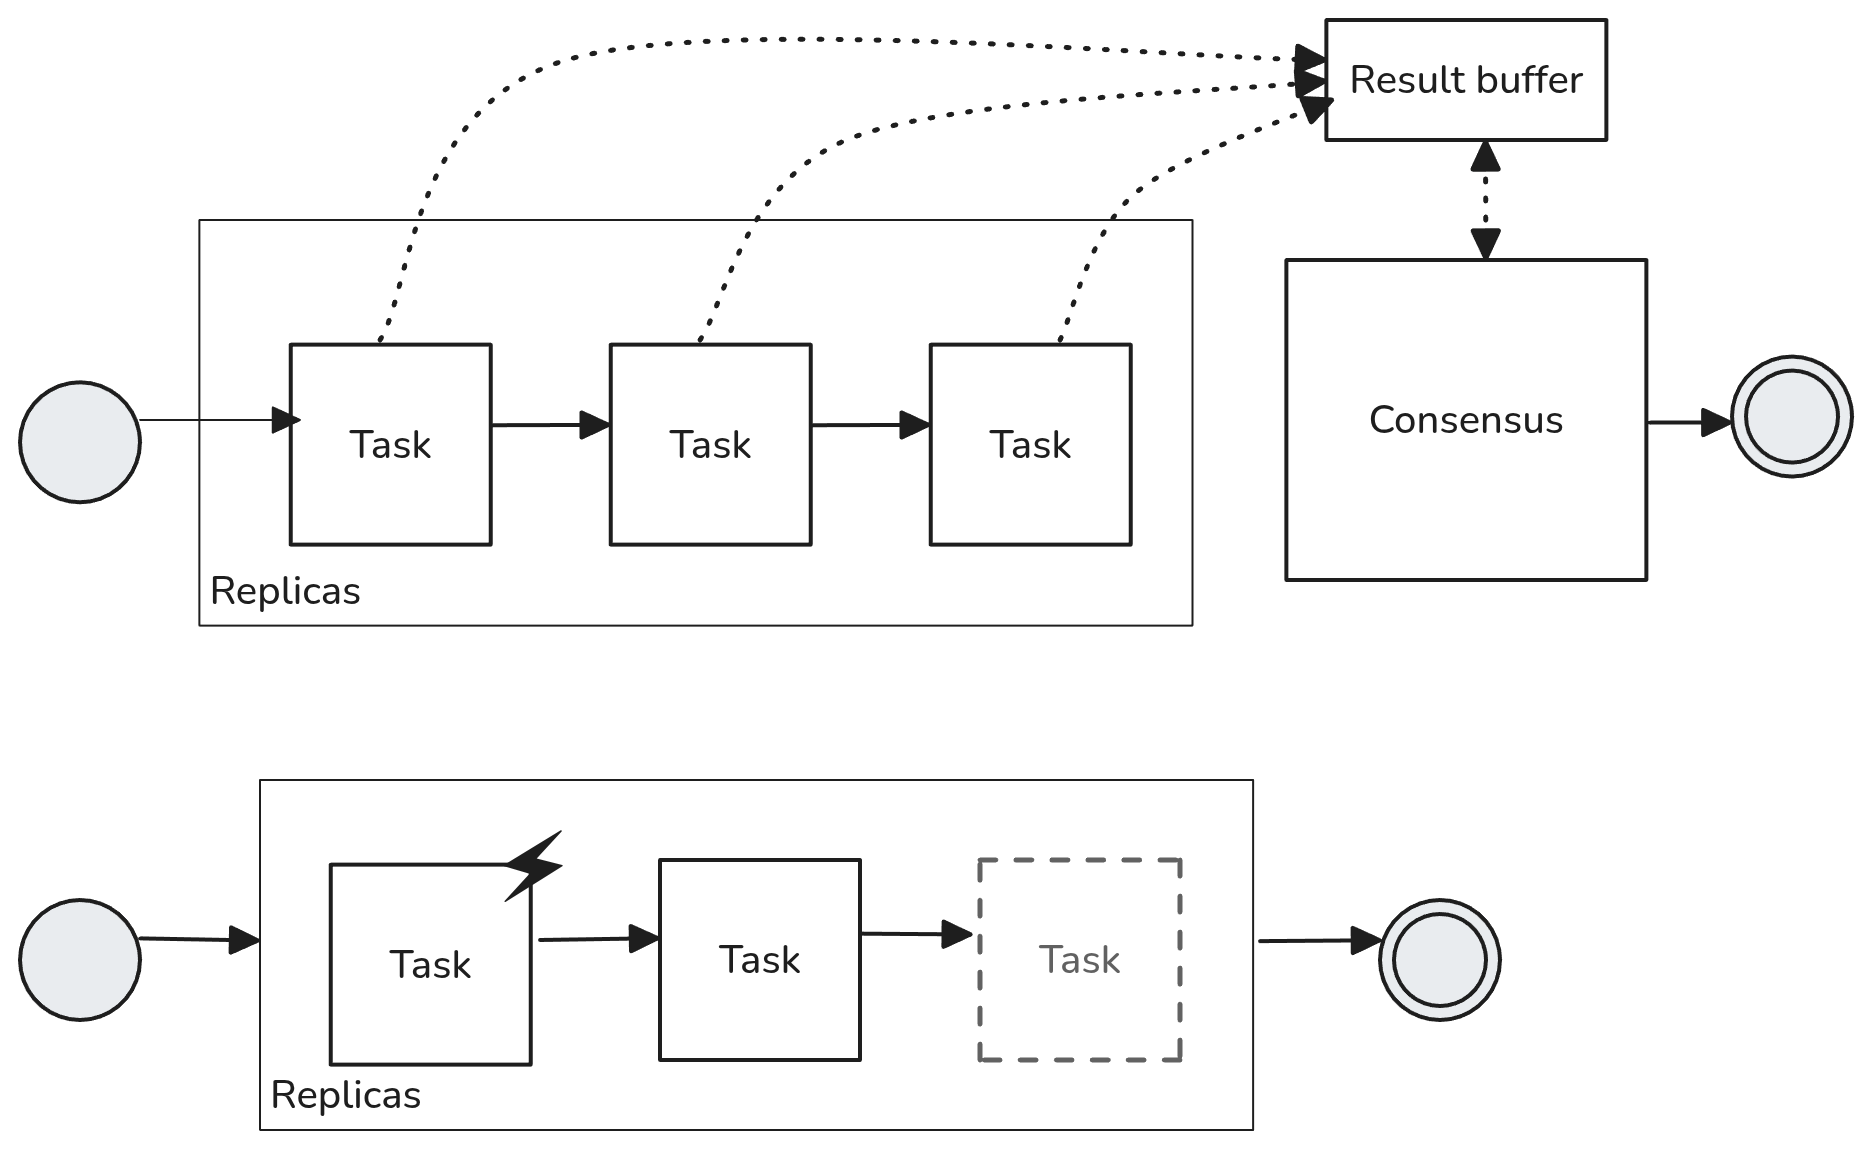
\includegraphics[width=1.0\textwidth]{assets/redundancia_reexec.png}
    \caption*{Fonte: Elaborada pelo autor}
    \label{fig:redundanciaReexec}
\end{figure}

Na \autoref{fig:redundanciaReexec} é possível observar a reexecução de uma tarefa em duas modalidades: Na primeira é realizado um consenso entre os resultados das execuções, e na segunda a tarefa é apenas reexecutada até $N$ vezes (podendo então tolerar até $N$ falhas transientes), encerrando sua execução caso nenhuma falha seja detectada. A segunda modalidade é particularmente útil para a implementação de condições de transparência \cite{SchedAndOptOfDistributedFT} que serão abordadas posteriormente.

% \renewcommand{\arraystretch}{1}
%  \begin{quadro}[H]
%     \centering
%     \caption{Comparação de trabalhos relacionados}
%     \label{tab:trabrel}
%     \begin{tabular}{|m{0.126\textwidth}|m{0.135\textwidth}|m{0.10\textwidth}|m{0.115\textwidth}|m{0.11\textwidth}|m{0.18\textwidth}|}
%         \hline
%         \rowcolor[HTML]{C0C0C0}
%         \textbf{Trabalho}  & \textbf{CNN base} & \textbf{Imagem} & \textbf{Tipo de Resolução} & \textbf{$\mu$C} & \textbf{Métricas} \\ \hline
        
%         \Centering\textbf{\citeDir{azami2022earth}}  & ShallowNet, LeNet e MiniVGGNet & RGB & Espacial e Espectral & Raspberry Pi 3+ & Acurácia \\ \hline
        
%         \Centering\textbf{\citeDir{maskey2020cubesatnet}}  & CubeSatNet & RGB & Espacial e Espectral & STM32H & Acurácia Global, \textit{F1-score} e Memória \\ \hline 
        
%         \Centering\textbf{\citeDir{leong2021unet}}  & U-net & RGB & Espacial e Espectral & STM32F7 & Precisão, Sensibilidade, Falso Negativo, Falso Positivo, Acurácia Global, \textit{F1-score} e Memória \\ \hline
        
%         \Centering\textbf{Este trabalho}  & LeNet-5 e HybridSN & HSI & Espectral & ESP32 e/ou Raspberry Pi Pico & Acurácia, F1-Score, Sensibilidade, Tempo de Processamento, Memória Utilizada, Potência Dissipada e Energia Consumida\\ \hline
%     \end{tabular}
%  \end{quadro}
%  \renewcommand{\arraystretch}{1}
 
